%%%%%%%%%%%%%%%%%%%%%%%%%%%%%%%%%%%%%%%%%
% Thin Sectioned Essay
% LaTeX Template
% Version 1.0 (3/8/13)
%
% This template has been downloaded from:
% http://www.LaTeXTemplates.com
%
% Original Author:
% Nicolas Diaz (nsdiaz@uc.cl) with extensive modifications by:
% Vel (vel@latextemplates.com)
%
% License:
% CC BY-NC-SA 3.0 (http://creativecommons.org/licenses/by-nc-sa/3.0/)
%
%%%%%%%%%%%%%%%%%%%%%%%%%%%%%%%%%%%%%%%%%

%----------------------------------------------------------------------------------------
%	PACKAGES AND OTHER DOCUMENT CONFIGURATIONS
%----------------------------------------------------------------------------------------

\documentclass[a4paper, 11pt]{article} % Font size (can be 10pt, 11pt or 12pt) and paper size (remove a4paper for US letter paper)

\usepackage[protrusion=true,expansion=true]{microtype} % Better typography
\usepackage[frenchb]{babel}
\usepackage{graphicx} % Required for including pictures
\usepackage{wrapfig} % Allows in-line images

\usepackage{mathpazo} % Use the Palatino font
\usepackage[utf8]{inputenc} % UTF-8 encoding for input, to get french special characters recognized
\usepackage[T1]{fontenc} % Required for accented characters
\linespread{1.05} % Change line spacing here, Palatino benefits from a slight increase by default
\usepackage{parskip} % add some space between paragraph

\makeatletter
\renewcommand\@biblabel[1]{\textbf{#1.}} % Change the square brackets for each bibliography item from '[1]' to '1.'
\renewcommand{\@listI}{\itemsep=0pt} % Reduce the space between items in the itemize and enumerate environments and the bibliography

\renewcommand{\maketitle}{ % Customize the title - do not edit title and author name here, see the TITLE block below
\begin{flushright} % Right align
{\LARGE\@title} % Increase the font size of the title

\vspace{50pt} % Some vertical space between the title and author name

{\large\@author} % Author name
\\\@date % Date

\vspace{40pt} % Some vertical space between the author block and abstract
\end{flushright}
}

%----------------------------------------------------------------------------------------
%	TITLE
%----------------------------------------------------------------------------------------

\title{\textbf{Techniques d'optimisation des temps de chargements dans les jeux à monde ouvert}\\ % Title
Ou comment réduire les temps de chargement} % Subtitle

\author{\textsc{Christian NGO \& Jonathan MULLER} % Author
\\{\textit{ESGI - 5ème année IJV}}} % Institution

\date{\today} % Date

%----------------------------------------------------------------------------------------

\begin{document}

\maketitle % Print the title section

%----------------------------------------------------------------------------------------
%	ABSTRACT AND KEYWORDS
%----------------------------------------------------------------------------------------

%\renewcommand{\abstractname}{Summary} % Uncomment to change the name of the abstract to something else

\begin{abstract}
Dans ce mémoire nous verrons comment réduire les temps de chargement des jeux vidéos en se basant à la fois sur les composants de la plateforme cible, sur les techniques de compression, sur l'algorithme et sur le level design.
\end{abstract}

\hspace*{3,6mm}\textit{Mots clefs:} chargement , optimisation , ressources , streaming , jeu % Keywords

\vspace{30pt} % Some vertical space between the abstract and first section

%----------------------------------------------------------------------------------------
%	ESSAY BODY
%----------------------------------------------------------------------------------------

\section*{Introduction}

Les jeux vidéos comportent année après année un nombre grandissant de ressources necessaire pour leur fonctionnement. Des textures aux modèles 3D, le poids de ces ressources augmente tout comme leur nombre, l'augmentation de la taillé mémoire des machines permettant aux créateurs de jeux de charger plus de ressources à la fois. Cependant, augmenter la taille et le nombre des ressources à un prix, celui du temps de chargement. Dans ce mémoire nous verrons comment réduire ces temps de chargement en s'adaptant aux médias qui permettent de stocker les ressources du jeu, en tirant partie des capacités des processeurs, de l'espace disponible et de la mémoire RAM, des différents formats de compression, mais aussi des adaptations de gameplay qui peuvent permettre un chargement transparant pour l'utilisateur.

%------------------------------------------------
\section*{Pourquoi avons nous besoin d'améliorer les temps de chargement ?}
La quantité de mémoire disponible augmente régulièrement sur les postes des utilisateurs, ce qui permet aux concepteurs de jeux de proposer des jeux de plus en plus riches et chargés en éléments graphiques, ce qui demande beaucoup de ressources à créer, stocker, et donc charger. En améliorant des temps de chargement des programmes, nous pouvons faire passer cette quantité de données en mémoire plus rapidement, et donc avoir des jeux qui permettent de jouer rapidement, sans passer de longs instants devant un écran de chargement à plusieurs reprises.

\section*{Comment influencer les temps de chargement}
Les temps de chargement peuvent être influencés de différentes manières.

Nous pouvons améliorer les temps de chargement en utilisant des techniques de stockage qui varient en fonction du média sur lequel le jeu est enregistré. Par exemple, les temps d'accès étant plutôt long sur un cd-rom, il faut veiller à limiter le nombre d'accès aux ressources et penser à charger des elements qui ne seront pas forcèment affichés tout de suite, lors des premiers chargements si la mémoire le permet.

Au contraire sur un disque SSD, les temps d'accès étant très bas et la capacité de transfert élevée, on pourra séparer les ressources dans des fichiers différents afin de les charger quasiement à la volée.

Les temps de chargement peuvent égallement être réduits en utilisant le processeur pour décompresser des ressources: ainsi le temps necessaire au transfert de la donnée depuis le disque à la mémoire est réduit puisque la donnée est compressée sur le dit disque. Il faut cependant que le mode de compression soit adapté à la puissance du processeur et à la vitesse de transmission du support de stockage.

En modifiant l'algorithme du jeu, nous pouvons aussi influer sur le chargement des données, en évitant par exemple de stocker plusieurs fois des ressources très similaires. Si nous prennons l'exemple des sprites 2D, nous pouvons stocker l'image de base une fois, puis effectuer toutes les déclinaisons de couleurs de manière algorithmique en modifiant la palette de couleurs. De cette façon, nous n'avons qu'à stocker une texture, puis uniquement des palettes de couleurs.

Enfin, une méthode pour cacher les chargements aux joueurs consiste à construire sont level design pour permettre certaines zones "tampons" comme un pont ou un couloir dont le passage est obligatoire pour passer d'une zone à l'autre, et qui va permettre de charger/décharger les zones concernées en tout transparence pour l'utilisateur. Cependant, cette technique est déconseillée puisqu'elle limite la liberté des level-designers en leur imposant des contraintes "techniques".

%------------------------------------------------
\section*{Optimisation par le matériel}
\subsection*{Benchmark des différents supports de stockage}
Pour mieux comprendre comment organiser nos ressources et la façon de les charger en fonction du support de stockage destiné au jeu, nous devons d'abord étudier et comprendre les deux principaux facteurs des temps de chargement liés au matériel: la vitesse de transfert et le temps d'accès. Le temps d'accès représente le temps écoulé entre le moment où la demande d'accès aux données va être effectuée et le début du transfert de cette donnée. Par exemple sur un disque dur, le temps que celui ci va prendre pour positionner sa tête de lecture, faire tourner le disque à la bonne position et commencer à lire la donnée. Le taux de transfert est le nombre de données qu'il est capable de faire transiter du support de stockage à la mémoire, par seconde.

\subsubsection*{Les CD-ROM}
\begin{wrapfigure}{r}{0.4\textwidth}
\begin{center}
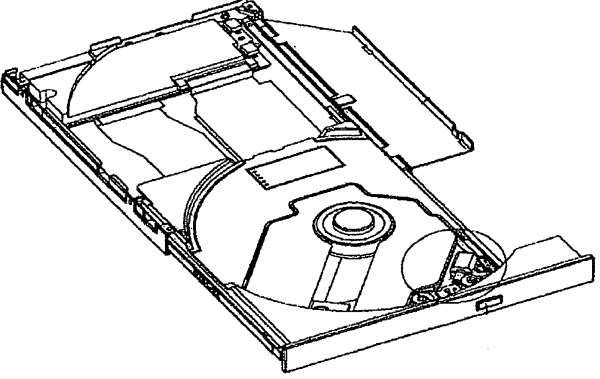
\includegraphics[width=0.38\textwidth]{images/cdrom.png}
\end{center}
\caption{Lecteur CD-ROM}
\end{wrapfigure}
Les CD-ROM ne sont plus beaucoup utilisés pour les jeux vidéos, qui dépassent maintenant souvent la capacité de stockage de ceux ci (entre 600 et 900Mo). Ils sont remplacés par des supports comme les DVD-ROM ou les Blueray. Cependant, il est intéressant d'étudier ce support de stockage pour une meilleur compréhension de l'évolution des périphériques.

Le CD-ROM a beaucoup été utilisé dans les années 90 et 2000, car le cout de fabrication de ce support est faible et ses capacité de stockage suffisantes, quitte à fournir régulièrement 4 CD-ROM dans les boites de jeu.

La vitesse de lecture de ce support est, par contre assez faible et rapidement les jeux ont utilisé ce média pour simplement installer les données sur le disque dur et servir de DRM.

Vitesse de transfert des lecteurs CD-ROM: \cite{hardware:cdromspeed}

\begin{tabular}{|l|c|c|}
  \hline
  Vitesse du lecteur & Taux de transfert (BPS) & Latence (ms)\\
  \hline
  Single-speed (1x)&153,600&400\\
	Double-speed (2x)&307,200&300\\
	Triple-speed (3x)&460,800&200\\
	Quad-speed (4x)&614,400&150\\
	Six-speed (6x)&921,600&150\\
	Eight-speed (8x)&1,228,800&100\\
	Ten speed (10x)&1,536,000&100\\
	Twelve speed (12x)&1,843,200&100\\
	Sixteen speed (16x)&2,457,600&90\\
	Eighteen speed (18x)&2,764,800&90\\
	Twenty four speed (24x)&3,686,400&90\\
	Thirty two speed (32x)&4,915,200&85\\
	One hundred speed (100x)&15,360,000&80\\
	CAV drives (12x - 24x)&1,843,200 - 3,686,400&150-90\\
  \hline
\end{tabular}

Comme nous pouvons le constater, les temps d'accès du lecteur CD-ROM sont assez élevé. Si nous devons charger 50 petits fichiers sur un lecteur 16x, nous ajoutons inutilement 4 secondes et demi de temps de chargement. Il convient donc d'encapsuler ces 50 fichiers dans un seul, de le charger d'une traite puis de faire la séparation des fichiers en mémoire.
C'est pour cette raison que sur les CD-ROMs de jeux nous trouvons souvent que peu de fichiers, mais qui prennent une grande partie de l'espace.

\subsubsection*{Lecteur DVD-ROM}
Le DVD-ROM a une vitesse 9 fois supérieure à celle d'un CD-ROM,\cite{hardware:dvdromspeed} pour une capacité allant de 4.7Go à 17.08Go (ce dernier étant très rare). Le temps d'accès aux données sur un DVD-ROM est d'environ 100ms pour les plus rapides, ce temps variant en fonction des lecteurs. Nous retrouvons donc avec les DVD-ROM le même problème qu'avec les CD-ROM: le temps d'accès au données élevé. Le taux de transfert et la quantité de données qu'il est possible de stocker sur celui ci en fait cependant un successeur de choix au CD-ROM, améliorant au passage les temps de chargement grâce à sa vitesse de lecture améliorée.

\subsubsection*{Lecteur BD-ROM}
Le BD-ROM est capable de transférer les données de 4.5Mo par seconde (x1) à 72Mo par seconde (x16)\cite{hardware:bdromspeed} et peut stocker entre 25Go et 50Go de données. Cela représente 50 fois la vitesse d'un CD-ROM. Bien que ses temps d'accès soient similaires voir plus grand que pour les DVD-ROMs, sa vitesse de transfert lui permet cependant de proposer des temps de chargements plus rapides, les données étant stockées sous forme de flux dans l'ordre d'utilisation comme pour les autres supports sous forme de disque, sa capacité de stockage permet en plus d’alléger le travail du processeur en proposant des données moins compressées.

\subsubsection*{Le Disque Dur}
\begin{wrapfigure}{r}{0.4\textwidth}
\begin{center}
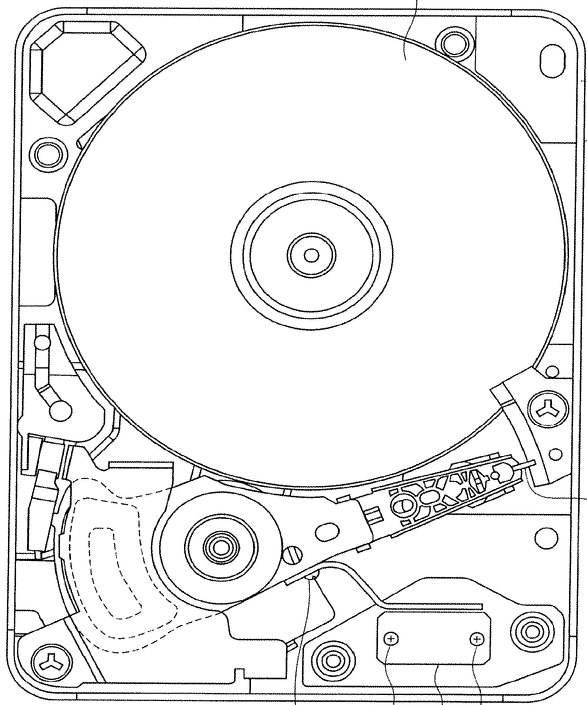
\includegraphics[width=0.38\textwidth]{images/hdd.png}
\end{center}
\caption{Lecteur CD-ROM}
\end{wrapfigure}
Le disque dur est le support de stockage le plus utilisé sur PC. Présent depuis les années 60 dans les ordinateurs de bureau, il a depuis continué à s'améliorer et à augmenter ses performances de lecture/écriture et ses temps d'accès. Le premier disque dur avait un temps d'accès de 600ms. Dès les années 80, ce temps a été réduit à 20ms et a continué de diminuer depuis.

Il existe 5 vitesses pour les disques durs, qui sont le nombre de rotation effectuées par le disque, par minute. Les vitesses de disque les plus rependues sont celles à 5400 tours/minute et 7200 tours/minute (respectivement 5.55ms et 4.16ms de temps d'accès moyen).\cite{hardware:hddspeed}

Les taux de transfert des disques à 7200 tours par minute en 2010 sont en moyenne de 125Mo par seconde. Comparé aux supports de stockage au format disque, le disque dur les surpasse tous. Cependant des problèmes peuvent intervenir sur les disques durs comme le corruption de données, ou la perte de vitesse à cause de la fragmentation qui peut intervenir sur certains systèmes de fichiers. Séparer les fichiers sur ce type de disque pour ne pas avoir de chargement sous forme de flux peut donc s'avérer pénalisant sur un disque fortement fragmenté.


\subsubsection*{Le SSD}
Le SSD est le support de stockage qui remplace peu à peu les disques durs. Ses taux d'accès étant très faible (en dessous de 0.1ms) et sa capacité de transfert élevé (entre 100 et 550Mo par seconde)\cite{hardware:ssdspeed}, il permet d'avoir peu voir pas de chargement visible pour l'utilisateur dans les jeux vidéos. 

Les caractéristiques du SSD sont proches de celles des cassettes de jeu vidéo utilisées sur les machines avant l'ère du CD. Ce type de support permet d'avoir des jeux où les chargements sont transparents pour l'utilisateur. De plus, la fragmentation des fichiers n'a aucun effet sur un disque SSD, les données peuvent donc être séparées pour minimiser le chargement de ressources inutiles et permettre un chargement à la volée rapide.

\subsubsection*{Multiplier les supports}
Si nous avons vu la supériorité des disques durs et SSD par rapport aux supports au format disque, nous pouvons quand même tirer partie du lecteur de disque pour améliorer encore les performances. Ainsi, nous pouvons nous servir du DVD/BD pour installer le jeu sur le disque dur, et garder une partie du disque qui servira lorsque le jeu sera lancé. Cela permettra d'accéder aux données à la fois du disque dur et sur le DVD/BD dans le jeu. C'est cette méthode qui est employée actuellement sur console, profitant du fait qu'elles soient équipées en disque dur pour réduire les temps de chargement.

%------------------------------------------------
%\section*{Optimisation par compression}

%------------------------------------------------
%\section*{Optimisation par algorithme}

%------------------------------------------------
%\section*{Optimisation par le level design}

%------------------------------------------------

%\section*{Conclusion}

%----------------------------------------------------------------------------------------
%	BIBLIOGRAPHY
%----------------------------------------------------------------------------------------

\bibliographystyle{unsrt}
\bibliography{References}

%----------------------------------------------------------------------------------------

\end{document}
